% !TEX root = ../thesis_main.tex
%
%
%
%%%% --- * --- %%%%	
\clearpage
\chapter{An Overview of Selected Techniques in Atomic Physics}
\label{atomicphysics_chapter}


%%%% --- * --- %%%%	
\section{The Shake-off Electron Spectrum}
\label{section:soe_intro}
Although the beta decay process is primarily concerned with the emission of beta particles (electrons or positrons) from a weak interaction that occurs within the nucleus, it is common for one or more \emph{orbital} electrons to also be lost in the process.  Although beta particles are emitted over a continuous energy spectrum, they commonly carry several MeV of kinetic energy.  By contrast, an atomic electron that becomes unbound in this process is likely to only carry a few eV of kinetic energy.  These are referred to as \acp{SOE}, since they are in some sense shaken off.

We will amend Eq.~\ref{eq:ourdecay} to reflect the presence of $N$ such \ac{SOE}s within each decay event, as
\bea
^{37}\textrm{K} &\rightarrow& \,^{37}\textrm{\!Ar}^{(N-1)+} + \beta^{+} + \nu_e + N \, e_{\textrm{SO}}, 
\label{eq:ourdecay_withsoe}
\eea
%\aside{Do I want to re-assign N somehow so the notation works better?}
where it is clear that, since the parent $^{37}\textrm{K}$ atom was electrically neutral before its decay by $\beta^+$ emission, the daughter $^{37}\textrm{\!Ar}$ will initially have an extra
%~\aside[jbn]{'extra' -> extra. You're not breaking charge conservation here, you don't need to define the word.} 
orbital electron (and therefore a negative net charge) if no electrons are shaken off.  We also note that it is common for multiple SOEs to be created in a given decay event.  

A further consideration is that the outer electron in an $^{37}\textrm{\!Ar}^{-}$ ion is not bound\cite{ArgonMinusIons}, and in an electric field such as is present within our experimental chamber, this outer electron is removed immediately to be accelerated through the field, leaving behind a neutral $^{37}\textrm{\!Ar}$ atom.  Although this is in principle a different physical loss mechanism, we will refer to unbound electrons resulting from either process as SOEs.  

It is useful to consider the energy spectrum of these shake-off electrons.  The most straightforward component of the SOE energy spectrum arises from the electrons that are lost immediately \emph{after} the decay, and we take these to initially have 0\,eV kinetic energy.  

For the shake-off electrons arising from nuclear decay process, the initial energy spectra for SOEs originating in a particular atomic orbital shell can be estimated according to the procedure outlined by J.S. Levinger in 1953~\cite{Levinger}.
%, who credits Feynman for the suggestion~\cite{Levinger}.
%%%~\note[done, nolist]{JB:  \\
%%%$\rightarrow$``by Levinger, who credits Feynman for the suggestion~\cite{Levinger}.''
%%%\\...\\
%%%(Since this is a true story that is not embellished by Feynman in someone else's joke book, but is in a footnote in the Physical Review,  I like to mention it.)
%%%}
%%%\note[done,nolist]{John says:  "the Feynman anecdote I did not relay correctly and should be cut"}
%%%\note[done,nolist]{btw2, you should drop ``who credits Feynman for the suggestion.''
%%%\\
%%%It turns out Feynman suggested how to do the recoil momentum dependence of the shakeoff, including in the sudden approximation an operator for a plane wave ofan electron moving at the recoil velocity. You are quite rightly not trying to consider this hard part here.
%%%}  \noindent
%
The strategy is to assume that the sudden approximation holds, meaning that the change in the shape of the potential well between initial and final states occurs so rapidly that the wavefunction of (in this case) the atomic electron does not have time to adapt.  Then, one simply calculates the overlap in wavefunctions between the bound initial state and the eigenstates of the final post-decay system.  The final state of the electron may be either bound or unbound, and analytic expressions to describe the energy of the unbound electrons may be obtained if the atom is treated as being hydrogenic --- as $^{37}\textrm{K}$ is an alkali, this treatment is well justified.
 
\note[done,nolist]{``On page 22, the ``sudden approximation'' is used but is never defined.''}
\note[done,nolist]{4. "sudden approximation"
\\...\\
You define it implicitly in text, but she didn't make the connection.
\\
It's worth defining it explicitly in passing instead: ``and simply calculate'' -> ``i.e. that one can calculate''
btw, `arising from the Weak process itself' confuses me, maybe say ``from the initial decay''
(i.e. as opposed to further atomic decays).}
%

Unfortunately, this treatment cannot determine the fractional contribution of each orbital to the total, nor can it determine the \emph{number} of electrons likely to be removed in a single decay event.  The implications of the SOE energy spectrum to the present experiment are discussed further in Chapter~\ref{sec:tof_bg}.

\note[org,nolist]{In the end, we used $(0.09)*(\textrm{0eV}) + (0.91)*(0.85*(\textrm{4S}) + 0.15*(\textrm{3P}))$.  But I say that in the other section.  Also, John used Eq.20 for the 4S, and Eq.24 for the 3P.}
\note{Comment on how well this matches our data?  Somehow?}

%\note{Should I talk about the distribution of how many SOEs come off in a decay?  I have measurements of the recoil charge distribution, which is related but not really the same thing.  From a theoretical POV, I don't know how many get shaken off.  Thankfully, it doesn't matter very much in the end.}

%%%%%\begin{figure}[h!!t]
%%%%%	\centering
%%%%%	\includegraphics[width=.999\linewidth]
%%%%%	{Figures/Levinger_SOETOF_prelim.pdf}
%%%%%	\note[clean]{Clean up SOE TOF pic in intro.  It doesn't show what I need!}

%\note[oldnote,nolist]{A picture of the SOE spectrum for the intro was here.  It's gone now, but it's important that we remember!  pretty sure I reference it from somewhere else...}

%%%%%	\note{Maybe just kill this picture?  At least reference it in the text somewhere.}
%%%%%	\caption[Levinger TOF]{Shake-off electron TOF (w.r.t. beta TOA) spectrum, showing how the spectrum is different if one includes different sets of initial electrons to be shaken off.  I forget why some of them have 0 eV.  Maybe those are the ones from the $\isotope[37]{Ar}^+$. ... Levinger TOF spectra for some different sets of SOE initial orbitals before shake-off.  (At least that's what it's supposed to be, after I fix the picture).  It's reconstructed event-by-event with beta times-of-flight that would pass some basic `good event' cuts.  Anyway, it turns out, it doesn't much matter what orbitals you lose SOEs from.  That's nice.  In the end, I used 85+15.  \comment{(Need to re-plot this.)} }	
%%%%%	\label{fig:levinger_TOF}
%%%%%\end{figure}



%%%% --- * --- %%%%	
%%%% --- * --- %%%%	
\section{Zeeman Splitting}
\label{sec:zeemansplitting}
In the presence of an external magnetic field $\vec{B}$, the Hamiltonian associated with an atom's orbital electrons will acquire an additional ``Zeeman Shift'' term, given by~\cite{corney}
\bea
\label{zeeman_hamiltonian}
H_{\mathrm{\,Zeeman}} &=& - \vec{\mu}\cdot \vec{B},
\eea
where $\vec{\mu}$ is the magnetic moment associated with the orbital under consideration.  In the limit where the magnetic field is too weak to significantly disrupt the coupling between the electron's spin- and orbital angular momenta, $\vec{\mu}$ may be treated as being fixed with respect to changes in the magnetic field.  It is this weak field regime which will be primarily of interest to us in work with magneto-optical traps.


With $\vec{\mu}$ fixed, it is clear that the magnitude of the energy shift must scale linearly with the strength of the magnetic field.  In considering the perturbation to the energy of a particular \emph{transition}, the perturbations to the initial and final states must of course be subtracted:
\bea
\Delta E_{\mathrm{\,transition}} &=& - \left( \vec{\mu}_f - \vec{\mu}_i \right) \cdot \vec{B}.
\eea 







%%% % % % %%%
\section{Optical Pumping}
\label{sec:op}
The optical pumping process necessary for this work involves using a laser to stimulate atomic transitions.  With a correctly tuned and polarized laser beam, the aggregate effect is to introduce a biased random walk towards a state of high spin-polarization (sometimes called a \emph{stretched state}).  Although the transitions to which the laser couples are often thought of as atomic transitions, the coupling of angular momenta between orbital electrons and the nucleus results in \emph{both} becoming polarized.  

With every absorbed photon, one unit of angular momentum is transferred to the atom, and an orbital electron jumps to a higher energy level.  By ensuring that the incident polarization laser is fully circularly polarized (and choosing an appropriate axis of quantization), it is possible to ensure that all the absorbed photons must \emph{increase} the angular momentum projection quantum number.  After absorbing a photon, the excited electron will eventually decay to a lower energy level, emitting a photon in the process.  The emitted photon carries one unit of angular momentum, and is emitted in a random direction -- therefore the resulting change in atomic angular momentum projection is also randomized, provided that there exists an available lower energy state for the orbital electron to decay into.   When the electron has been moved to the maximally polarized ground state, it can no longer be excited by the laser beam that drove it there (assuming perfect circular polarization for the laser), because there is no excited state available with higher angular momentum.  

Given that the process is accurately modeled as a biased random walk towards a particular state, it should be clear that once a majority of the atoms have arrived at the stretched state, the optical pumping process has progressively diminishing returns, as there are fewer and fewer unpolarized atoms available to be polarized.  As a practical matter, the entire process takes several microseconds before the system arrives at something of a steady state, with depolarizing forces balanced against the optical pumping rate.

We now consider the two primary depolarization mechanisms.  The first and most straightforward of these arises as a result of incomplete circular polarization in the optical pumping laser.  The overall laser polarization can be represented as a linear combination of left-handed and right-handed ($\sigma_{\pm}$) circularly polarized components.  If the $\sigma_{+}$ light \emph{increases} the angular momentum projection in the atomic system on which it is incident, then the $\sigma_{+}$ light must necessarily \emph{decrease} that same quantity.  In practice, it is impossible to completely polarize the optical pumping laser, so it is inevitable that there will be some depolarizing component, however small, within the optical pumping laser.

The cloud polarization can also be disrupted by the presence of a non-uniform magnetic field as the result of Larmor precession.  In a simplified semi-classical picture (which translates remarkably well to the quantum mechanical reality), this would result in any spins that are not fully aligned (or anti-aligned) with the magnetic field precessing about the local magnetic field lines.  If the magnetic field is aligned with the intended axis of polarization, the spins will precess, but the overall polarization (ie, the spin projection onto the selected axis) will be unchanged.  

By contrast, if the magnetic field is misaligned with the polarization axis, then a spin (even one initially aligned with the polarization axis) will experience a time-dependent depolarization force as it precesses.  Worse yet, if the magnetic field is non-uniform, then the spins on one side of the atom cloud will precess about a different axis, at a different rate, than the spins on the opposite side.  

This time-dependent depolarization mechanism is critical to \ac{NMR} measurements, but for our purposes here, we wish to suppress it.  To minimize depolarization effects arising from magnetic field non-uniformities, an additional uniform magnetic field may be applied along the axis of polarization.  This has the effect of decreasing the \emph{fractional} size of any non-uniformities that may be present.  The applied field must also be kept relatively small ($\sim$ 2.3 Gauss, in our case) in order to prevent the atomic and nuclear angular momenta from becoming decoupled.  



\note[note,nolist]{}


\note[note,nolist]{}

\color{skyblue}
The primary detail described here is that the optical pumping is disturbed by any component of magnetic field not directed along the quantization axis --- in our case, the vertical axis, defined by the direction of propogation for the optical pumping light, and along which the detectors are placed.  The optical pumping process is described in detail within our collaboration's Ref.~\cite{ben_OP}, and the required sophistication with an AC-MOT described in Section~\ref{sec:acmot} below.
\color{black}





%%% % % % %%%
%%% % % % %%%
%%% % % % %%%
\section{Doppler Cooling}
\label{sec:dopplercooling}
We consider a setup in which a cloud of two-level atoms lies along the path of two counter-propagating laser beams, both tuned to
resonance.  For simplicity, we treat this cloud as being one dimensional along the axis of laser propagation.  
With two counter-propagating laser beams of equal intensity and detuning,
\aside{...and opposite polarization.  Or something.  I have to talk about the selection rules somewhere else.} 
the ``push'' from interaction with one beam is, on average within the lab frame, perfectly counteracted by the push from the opposite-propagating beam, so there is no net velocity transfer to a cloud initially at rest.  These pushes, however, are applied on the level of the individual atom, and are the result of individual photons being absorbed and emitted.  Because this process is probabilistic rather than deterministic, each individual atom will undergo a random walk.  

We now consider the effect of detuning on this process.  We will suppose that both lasers are equally detuned slightly to the red of resonance.  This will obviously decrease absorption by atoms at rest within the lasers' path -- however the atoms within the cloud are not at rest, but rather are undergoing thermal motion.  As such, within the rest frame of each individual atom, the two laser beams will appear to be Doppler shifted in opposite directions, with the sign dependent on atomic motion.  In particular, atoms moving against a laser's direction of propagation will see that laser beam as being blueshifted within their own rest frame.  Since the laser was redshifted relative to resonance within the lab frame, adding an additional blueshift will serve to bring the photons' energy back towards resonance, making them more likely to be absorbed.  For this same atom, the laser propagating in the same (lab frame) direction as the atom itself will appear further redshifted, and its photons are less likely to be absorped.  

The result of many such atom-photon interactions is that an individual atom, no matter which way it's moving at any given time, will absorb more photons from the direction where the momentum transfer slows them down, and fewer from the direction where the momentum transfer speeds them up.  In short, each individual atom is \emph{greatly} slowed down.  At the macroscopic level, this translates to a decrease in the \emph{temperature} of the atom cloud.  Such a setup is sometimes referred to as a (one-dimensional) ``optical molasses'' due to the viscous drag force induced on atomic motion, and it is straightforward to extend this model to three dimensions.

Although this setup will decrease atomic velocity, it does not create a confining force, so (eg, in three dimensions) the atoms are still free to move out of the lasers' path, albeit at a decreased speed.
\note{...This will slow the atom down, at least up to a limit related to the linewidth of the atomic transition and/or the laser.  There's something to look up.}






%%% % % % %%%
%%% % % % %%%
%%% % % % %%%
\section{Atom Trapping with a Magneto-Optical Trap}
\label{section:mot}
\note[note]{Move(d) the content of the other MOT section into here.}
Since its initial description by Raab et. al. in 1987~\cite{raabprentiss}, the \ac{MOT} has become a widely used technique in many atomic physics laboratories.\aside{An opportunity to cite a bunch of people here...} The MOT produces confined samples of cold, electrically neutral and isotopically pure atoms confined within a small spatial region.  It is these properties that make the MOT a valuable tool not only in atomic physics, but for precision measurements in nuclear physics as well, and the \ac{TRINAT} collaboration has adopted the technique wholeheartedly.

The technique is used predominantly with alkalis due to their simple orbital electron structure, and once set up it is quite robust.  The MOT's trapping force is specific to the isotope for which the trap has been tuned. This feature makes it ideal for use in precision radioactive decay experiments, since the daughters are unaffected by the trapping forces keeping the parent confined.

A \ac{MOT} combines the slowing features of an optical molasses (Sec.~\ref{sec:dopplercooling}) with the Zeeman splitting (Sec.~\ref{sec:zeemansplitting}) arising from a quadrupolar magnetic field to produce a robust and isotope-specific trapping force in all three dimensions.  

A MOT can be created from relatively simple components:  a quadrupole-shaped magnetic field, typically generated by two current-carrying coils of wire\aside{anti-helmholtz, motherfucker.}, and a circularly polarized laser tuned to match one or more atomic transitions in the isotope of interest.  Because a MOT is easily disrupted by interactions with untrapped atoms, the trap must be created within a vaccuum system.  Finally, a source of atoms to be trapped is required.  See Fig.~\ref{fig:mot}.

%In order to understand the mechanism by which a MOT is able to confine atoms, we must first introduce the Zeeman effect (Section~\ref{sec:zeemansplitting}) and a description of an optical molasses (Section~\ref{sec:dopplercooling}). A functional MOT combines the forces resulting from these two physical effects to trap and cool atoms.


%%% % % % %%%
%\section{Atom Trapping with a MOT (tbd) }
\note[note]{Move this content over to the *other* MOT section.}
The quadrupolar magnetic field\aside{constant field gradient} is typically generated using a set of two current carrying electrical coils in a geometry similar to a Helmholtz coil, but with the two coils' currents flowing anti-parallel to one another.  This anti-Helmholtz coil is constructed to surround the trapping region, and introduces a quadrupolar magnetic field.  Within the central region where the trap is located, the magnetic field $\vec{B}$ has the approximate shape,
\bea
	\vec{B} &=& 2 B_0 z \,\hat{z} - (B_0 x \,\hat{x} + B_0 y \,\hat{y}), 
\eea
where $B_0$ represents the overall strength of the magnetic field, $\hat{x}$, $\hat{y}$, and $\hat{z}$ are coordinate unit vectors such that the $\hat{z}$ axis points along the axis of the anti-Helmholz coil, and $x$, $y$, and $z$ represent the position (relative to the central point between the two coils) at which the magnetic field is being described.
In particular, this implies that the field magnitude is zero at the centre, and increases linearly in every direction as one moves away from the centre.

The retroreflecting lasers are red-detuned and circularly polarized in a direction selected to couple to the Zeeman shifted energy level which will push a given atom towards the centre.  This provides a restoring force in all three dimensions to atoms that have moved too far from the centre.  See Fig.~\ref{fig:mot}.

\begin{figure}[h!!!!!t!b]
	\centering
		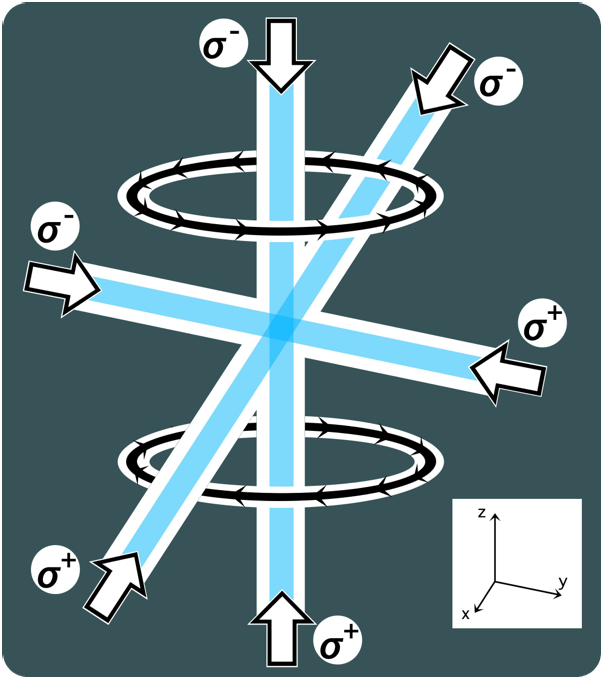
\includegraphics[width=.999\linewidth]{mot.png}
		\caption[Components of a Magneto-Optical Trap]{Components of a magneto-optical trap, including counterpropagating circularly polarized laser beams (with $\sigma^\pm$ polarization) intersecting at the centre, and current-carrying electrical coils above and below the central intersection point, used to generate a magnetic field gradient.  With antiparallel currents, the magnitude of the field in the region near the centre is linear in all directions.  Diagram taken from~\cite{thesis}}.
		\label{fig:mot}
    	\label{fig:themot}
\end{figure}


%%% % % % %%%
%%% % % % %%%
%%% % % % %%%
\section{The AC-MOT}
\label{sec:acmot}
%\note[done,nolist]{Initially, this section is a literal duplicate of Chapter~\ref{section:acmot_and_polarization}.  When I'm done, most of the content will live *there*.  This is the intro chapter/section here.}
%
One specialized type of magneto-optical trap, the AC-MOT, allows for the trap's magnetic field to be rapidly shut off.  First described by Harvey and Murray in 2008~\cite{harveymurray}, the AC-MOT is so named because of the sinusoidal alternating current (AC) used in its anti-Helmholtz coils --- in contrast to the constant direct current used in a typical MOT (hereafter referred to as a DC-MOT to eliminate ambiguity).  Although the DC-MOT's robust trapping mechanism cannot be fully matched by a similar AC-MOT, the DC-MOT is very slow to turn off, and it is this latter consideration that has led the TRINAT collaboration to implement an AC-MOT in its second trap.

%, a consideration that led the TRINAT collaboration to implement an AC-MOT  
%It was this consideration that motivated the TRINAT collaboration to implement an 
%It is this consideration 
%As a result, the TRINAT collaboration has 

Although the trapping mechanism itself can be rapidly destroyed in both an AC- and DC-MOT by simply shutting off the trapping lasers, the DC-MOT's magnetic field is comparatively slow to dissipate and challenging to control during this time.  Because the optical pumping process 
necessary to spin-polarize the atoms 
%which (in the present experiment) immediately follows the MOT being shut off 
requires a uniform magnetic field 
over the region of interest 
(in contrast to the uniform magnetic field \emph{gradient} needed for a functional MOT), we do not consider the MOT to have been fully shut off until any residual magnetic fields have completely dissipated.  
Put another way, 
for optical pumping, a weak dipole-shaped magnetic field is preferred, and this is not possible while the MOT's quadrupole field is in place.  %the quadrupole field has not dissipated.

With the DC-MOT designed to operate continuously, 
it should be unsurprising that it 
%and as such 
is fairly slow to turn off.  The limiting factor is the speed at which the magnetic field can be eliminated; it is particularly problematic when electrically conductive materials are present nearby, as is the case for our experimental chamber.  
%and in the presence of electrically conductive materials especially, the magnetic field can take a (comparatively) long time to dissipate.  
%This is problematic for an experiment such as this one, 
This is because a rapidly changing magnetic field will necessarily induce an electrical potential, producing a current in any nearby conductors.  These induced eddy currents will, themselves, produce a magnetic field and further eddy currents as that magnetic field dissipates.  The result is a magnetic field which is slow to dissipate and difficult to control during the dissipation process.  In general, the atoms do not remain reliably confined while the magnetic field dissipates, as the field during this time may include anomalies which could result in atoms actively being pushed out of the trap by the trapping lasers.  For similar reasons, the atoms also cannot be successfully polarized during this time period.  

It is clearly important that as little time as possible be wasted in this intermediate stage where the atoms can neither be confined nor polarized.  The more straightforward reason behind this is simply that any time wasted during beamtime is data lost.  A slightly more subtle but related reason is that when the trapping mechanism is removed, the atom cloud undergoes thermal expansion ($\sim$1\,mK).  If the cloud is retrapped quickly enough, the whole process can be done with minimal atom loss --- however once the cloud has dissipated it cannot be re-trapped, as the trapping forces act on only a small spatial region.

The principle behind the AC-MOT is to simply run a sinusoidal current through one's anti-Helmholtz coils while flipping the laser polarization to remain in sync with the magnetic field.  Crucially, the phase of the magnetic field will lag somewhat behind the phase of the current in the anti-Helmholtz coils, as a result of induced eddy currents in nearby materials.  The precise amount of phase lag in a given system is a function both of the geometry and electrical impedence properties of the nearby materials, as well as the frequency of the sinusoid.  

\note[note]{}
%\note[note]{Above, everything is re-edited for its current thesis location.  
%\\
%Below, shit's still basically duplicated in that other section.}
\note[note]{Put that *other* AC-MOT figure here.}

%The AC-MOT was first described by Harvey and Murray~\cite{harveymurray}, but the TRINAT collaboration has adopted its use because it enables the polarization-destroying magnetic field to be eliminated quickly after the MOT is shut off.  Some details of the present implementation of the AC-MOT are given in Ref.~\cite{thesis}, done with a separate MOT geometry from this beta decay work.  A diagram of showing the operation phases of several key components in our AC-MOT/optical pumping duty cycle is shown in Fig.~\ref{fig:acmot}.

%%%%%\begin{figure}[ht]
%%%%%	\centering
%%%%%		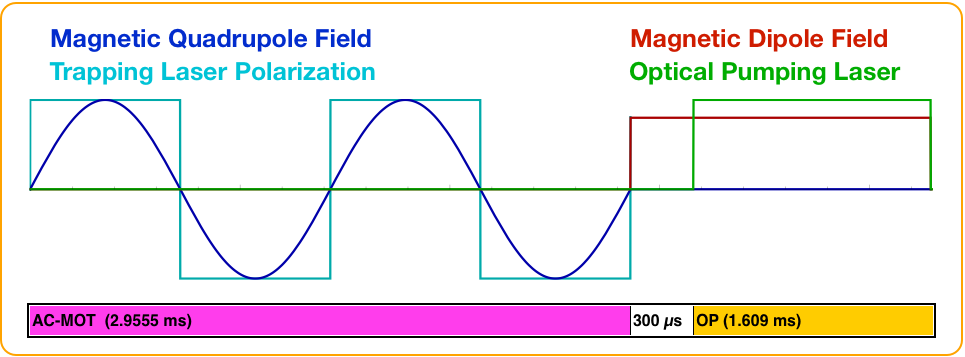
\includegraphics[width=.999\linewidth]{acmot.png}
%%%%%		\caption[The AC-MOT and Optical Pumping Cycle]{One cycle of trapping with the AC-MOT, followed by optical pumping to spin-polarize the atoms.  After atoms are transferred into the science chamber, this cycle is repeated 100 times before the next transfer.  The magnetic dipole field is created by running parallel (rather than anti-parallel as is needed for the MOT) currents through the two coils.}
%%%%%		\label{fig:acmot}
%%%%%\end{figure}
%%
%%A standard DC-MOT operates continuously, and in the presence of electrically conductive materials especially, the magnetic field can take a (comparatively) long time to dissipate.  This is problematic for an experiment such as this one, because the atoms do not remain confined while the magnetic field dissipates due to potential anomalies in the magnetic field shape arising from induced eddy currents, and for similar reasons, they cannot be successfully optically pumped during this time period either.  Therefore, it is important to waste as little time as possible switching between the MOT and the  optical pumping phases in the duty cycle.  For optical pumping, a weak, dipole-shaped magnetic field is preferred, and this is not possible while the quadrupole field has not dissipated.


\note{Eddy currents in your nearby metal objects will still be produced, and these changing eddy currents will \emph{also} create a sinusoidally oscillating magnetic field.  If correctly timed, it is possible to eliminate the current in the anti-Helmholtz coils at the precise time when the eddy currents are also eliminated.  This process can easily reduce the size of any eddy currents still produced by around an order of magnitude or more, and these remaining eddy currents decay more rapidly as well.}

%\note{This content *came from* that other section, and needs to go in here somewhere:  ``Many laser ports to make the MOT functional, and for optical pumping.  Fancy mirror geometry to combine optical pumping and trapping light along the vertical axis.  Water-cooled (anti-)Helmholz coils within the chamber for the AC-MOT, fast switching to produce an optical pumping field.''  }

\note{... Sadly, this also removes our trapping mechanism.  We could keep the optical molasses after the field is off if we wanted to, but we don't, because we wouldn't be able to optically pump the atoms then.  But at least the atoms are cold-ish (we can measure!  I think it's done indirectly in that one table, or for realsies in Ben's thesis), so we can let them just chill for a little while before we have to re-trap them.  Don't lose too much.  (How much do we lose?  Have we quantified that somewhere?  Probably.).  ...}

%\note[note]{Probably document things about the waveform and frequency used for the beamtime, since I don't think it's in my MSc.}

%As alluded to in the previous section~(\ref{section:overview}), the measurements in question required a spin-polarized sample of atoms, and a precise knowledge of what that polarization was.  This is needed in order to make best use of the superratio asymmetry for both $\Abeta$ and $\bFierz$ measurements.~\cite{ben_Abeta}\cite{ben_OP}.

%A MOT requires a quadrupolar magnetic field, and we generate ours with two current-carrying anti-Helmholtz coils located within the vacuum chamber itself.  Since these coils are expected to run an alternating current, heat is produced and cannot be dissipated in the vacuum.  Therefore the coils themselves are hollow copper tubes, and they are continuously cooled by pumping temperature-controlled water through them.   


%\note{Note that because the atoms within a MOT can be treated as following a thermal distribution, some fraction of the fastest atoms continuously escape from the trap's potential well.  Even with the most carefully-tuned apparatus, the AC-MOT cannot quite match a similar standard MOT in terms of retaining atoms.  The TRINAT AC-MOT has a `trapping half-life' of around 6 seconds, and although that may not be particularly impressive by the standards of other MOTs, it is more than adequate for our purposes.  $^{37}\textrm{K}$ itself has a radioactive half-life of only 1.6 seconds 
%(cite someone), so our dominant loss mechanism is radioactive decay rather than thermal escape. }


%We spin-polarize $^{37}\textrm{K}$ atoms within the trapping region by optical pumping~\cite{ben_OP}.  A circularly polarized laser is tuned to match the relevant atomic resonances, and is directed through the trapping region along the vertical axis in both directions.  When a photon is absorbed by an atom, the atom transitions to an excited state and its total angular momentum (electron spin + orbital + nuclear spin) along the vertical axis is incremented by one unit.  When the atom is de-excited a photon is emitted isotropically, 
%so it follows that if there are available states of higher and lower angular momentum, the \emph{average} change in the angular momentum projection is zero.  If the atom is not yet spin-polarized, it can absorb and re-emit another photon, following a biased random walk towards complete polarization.  
%
%In order to optimally polarize a sample of atoms by this method, it is necessary to have precise control over the magnetic field.  This is because absent other forces, a spin will undergo Larmor precession about the magnetic field lines.  In particular, the magnetic field must be aligned along the polarization axis (otherwise the tendency will be to actually depolarize the atoms), and it must be uniform in both magnitude and direction over the region of interest to avoid introducing a spatially-dependent depolarization mechanism.  
%Note that this type of magnetic field is not compatible with the MOT, which requires a uniform magnetic field \emph{gradient} in all directions (characteristic of a quadrupolar field shape), and has necessitated our use of the AC-MOT.
%
%In the end, the average (over both directions) polarization $|\vec{P}|$ achieved during the 2014 beam time is $|\vec{P}| = 0.9913 \pm 0.0009$, and the measurements are consistent with both polarization directions having the same magnitude of polarization\cite{ben_OP}.
%
%\note[tag, nolist]{End duplicated section.  When I'm done, most of the content should live *over there*.}


%%%\section{Zeeman Slowing}
%%%\label{sec:zeeman}
%%%
%%%\note[note]{Yeah, uh, from a theoretical point of view, this is basically the same shit as doppler cooling, right?}
%%%
